\chapter{Auswertung}
\section{Flussdichte}
Die mittlere Strecke entlang des Eisenkerns beträgt
\begin{equation}
    \bar{s_{Fe}} = 2 \cdot (\SI{139,95}{mm} + \SI{101,7}{mm} + 2 \cdot \SI{30}{mm}) - \SI{7,2}{mm} = \SI{596,1}{mm}
\end{equation}
Die des Luftspaltes ist trivial und beträgt \(s_L=\SI{7,2}{mm}\) (vgl. \cref{fig:zeichnungKern}).
\par\medskip
Der sich für einen Spulenstrom von \SI{2,4}{A} einstellende Fluss berechnet sich mit Hilfe der Gleichungen \cref{eq:NI}
bis \cref{eq:Rm} zu
\begin{gather}
    N \cdot I_S = \Phi \cdot \left(\frac{\bar{s_{Fe}}}{\mu_o\mu_{r,Fe}A} + \frac{s_L}{\mu_0 A}\right) \nonumber \\
    \Leftrightarrow \nonumber \\
    \Phi = N \cdot I_S \cdot A \cdot \mu_0 \cdot \left(\frac{\bar{s_{Fe}}}{\mu_{r,Fe}} + s_L\right)^{-1}
    \label{eq:fluss}
\end{gather}
Durchdringt der magnetische Fluss eine ebene Fläche entlang ihrer Normalen ist die Flussdichte dargestellt durch
\begin{equation}
    B = \frac{\Phi}{A}
    \label{eq:flussdichte}
\end{equation}
Im vorliegenden Fall ist die Fläche über die gesamte Strecke konstant. \cref{eq:flussdichte} in \cref{eq:fluss} eingesetzt
verschwindet die Fläche. Mit den Werten \(\mu_{r,Fe}=500\), \(\bar{s_{Fe}}=\SI{596,1}{mm}\), \(s_L=\SI{7,2}{mm}\), \(n=300\),
\(I_S=\SI{2,4}{A}\) und um den Faktor \(2\) multipliziert ergibt sich so eine rechnerische Flussdichte von
\begin{align}
    B &= 2 \cdot \frac{n \cdot I_S \cdot \mu_0}{\left( \frac{\bar{S_{Fe}}}{\mu_{r,Fe}}\right) + s_L} \nonumber \\
    &= 2\cdot \frac{300 \cdot \SI{2,4}{A} \cdot 4\pi \cdot \SI{10^{-7}}{\volt\second\per\ampere\per\metre}}{ \left( \frac{\SI{0,5961}{m}}{500} \right) + \SI{0,0072}{m} } \nonumber \\
    &\approx \SI{215,624}{mT}
\end{align}
Der Faktor \(2\) trägt der Tatsache Rechnung, dass im vorliegenden Aufbau zwei Spulen mitläufig angeordnet und verschaltet
sind.
\par
Der rechnerische Wert für die Flussdichte weicht um etwa \SI{32}{mT} vom messtechnisch ermittelten Wert ab. Die Differenz
lässt sich durch Vereinfachungen der Gleichung, so wie durch Toleranzen im Messaufbau erklären.
%
%==================================================================
%
\section{Probenparameter}
\begin{figure}[H]
    \centering
    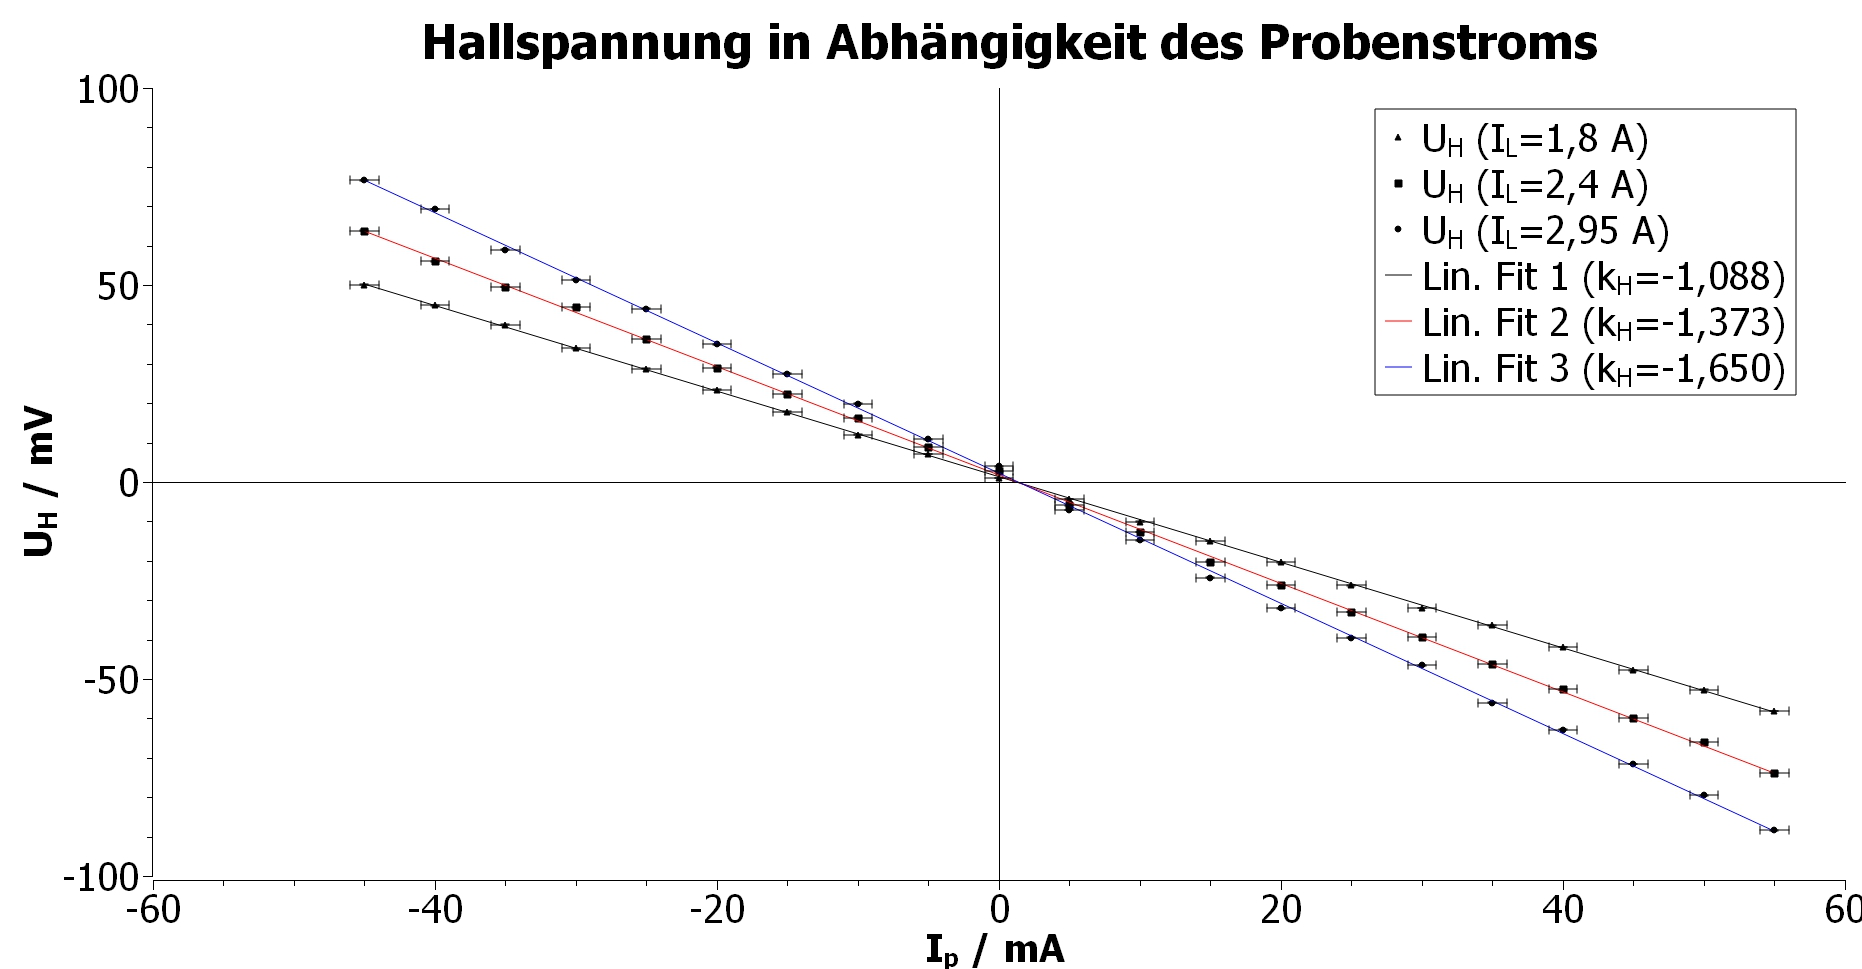
\includegraphics[width=\textwidth]{scidavis/abbildungen/hallspannung.jpeg}
    \caption[Diagram der Messwerte $U_H(I_p)$]{Gemessene Hallspannung $U_H$ aufgetragen über den Probenstrom $I_p$ für drei verschiedene Spulenspannungen $I_L$.}%
    \label{fig:hallspannung}
\end{figure}

Der \textsc{Hall}-Koeffizient ist mit \(A_H = (qn_q)^{-1}\) ein materialabhängiger Parameter und dient als Proportionalitätsfaktor der \textsc{Hall}-Spannung \(U_H\).
Aus \cref{eq:UH2} lässt er sich bestimmen durch
\begin{equation}
   A_H = \frac{U_H \cdot b}{B \cdot I_p} = \frac{k_H \cdot b}{B} = \frac{1}{q \cdot n_q}%
   \label{eq:hallKoeff}
\end{equation}
\(k_i\) sind hier die Steigungen des \(U_H(I_p)\)-Diagramms mit den zugehörigen Flussdichten \(B_i\).
Daraus ergibt sich ein mittlerer wert für den \textsc{Hall}-Koeffizienten zu
\begin{equation}
    A_H = \frac{\SI{-1,373}{\volt\per\ampere} \cdot \SI{0,001}{m}}{\SI{0,248}{T}}
    \approx \SI{-5,5 \cdot 10^{-3}}{\metre\cubed\per\ampere\per\second}
\end{equation}
mit einer Unsicherheit von
\begin{align}
    \Delta A_H &= \left| \partial A_H \over \partial k_H \right| \cdot \Delta k_H + \left| \partial A_H \over \partial h \right| \cdot \Delta h + \left| \partial A_H \over \partial B \right| \cdot \Delta B \nonumber \\
    &= \left| \frac{h}{B} \right| \cdot \Delta k_H + \left| \frac{k_H}{B} \right| \cdot \Delta h + \left| \frac{k_H \cdot h}{B^2} \right| \cdot \Delta B \nonumber \\
    &= 
    \frac{\SI{0,01}{m}}{\SI{0,248}{T}} \cdot \SI{0,0049}{\volt\per\ampere} + 
    \frac{\SI{1,373}{\volt\per\ampere}}{\SI{0,248}{T}} \cdot \SI{10^{-4}}{m} + 
    \frac{\SI{1,373}{\volt\per\ampere} \cdot \SI{10^{-3}}{m}}{\SI{0,248^2}{T^2}} \cdot \SI{10^{-4}}{T} \nonumber \\
    &= \pm \SI{0,8 \cdot 10^{-3}}{\metre\cubed\per\ampere\per\second}
\end{align}
\par\medskip
Die Ladungsträgerkonzentration \(n_q\) lässt sich analog dazu berechnen durch
\begin{align}
    n_q &= \frac{B}{k_H \cdot q \cdot b} \nonumber \\
    &= -\frac{\SI{0,248}{T}}{\SI{1,602}{As} \cdot \SI{0,001}{m} \cdot \SI{1,373}{\volt\per\ampere}} \cdot 10^{19} \nonumber \\
    &\approx \SI{1,128 \cdot 10^{21}}{m^{-3}}
\end{align}
Der Fehler beträgt hier
\begin{align}
    \Delta n_q &=
    \left| \frac{\partial n_q}{\partial b} \right| \cdot \Delta b +
    \left| \frac{\partial n_q}{\partial B} \right| \cdot \Delta B +
    \left| \frac{\partial n_q}{\partial k_H} \right| \cdot \Delta k_H \nonumber \\
    &= \left| \frac{B}{k_H \cdot q \cdot b^2} \right| \cdot \Delta b +
    \left| \frac{1}{k_H \cdot q \cdot b} \right| \cdot \Delta B +
    \left| \frac{B}{k_H^2 \cdot q \cdot b} \right| \cdot \Delta k_H \nonumber \\
    &= \frac{10^{19}}{\SI{1,602}{As}} \cdot \Bigg[\left( \frac{\SI{0,248}{T}}{\SI{1,373}{\volt\per\ampere} \cdot \SI{10^{-6}}{m^2}} \right) \cdot \SI{10^{-4}}{m}
    + \left( \frac{1}{\SI{1,373}{\volt\per\ampere} \cdot \SI{10^{-3}}{m}} \right) \cdot \SI{10^{-4}}{T} \nonumber \\
    &\quad + \left( \frac{\SI{0,248}{T}}{ \left( \SI{1,373}{\volt\per\ampere} \right)^2 \cdot \SI{10^{-3}}{m}} \right) \cdot 4,9 \cdot \SI{10^{-3}}{\volt\per\ampere} \Bigg] \nonumber \\
    &= \pm 1,173 \cdot \SI{10^{20}}{m^{-3}}
\end{align}

\par\medskip
%
%===================================================================
%
\begin{figure}[H]
    \centering
    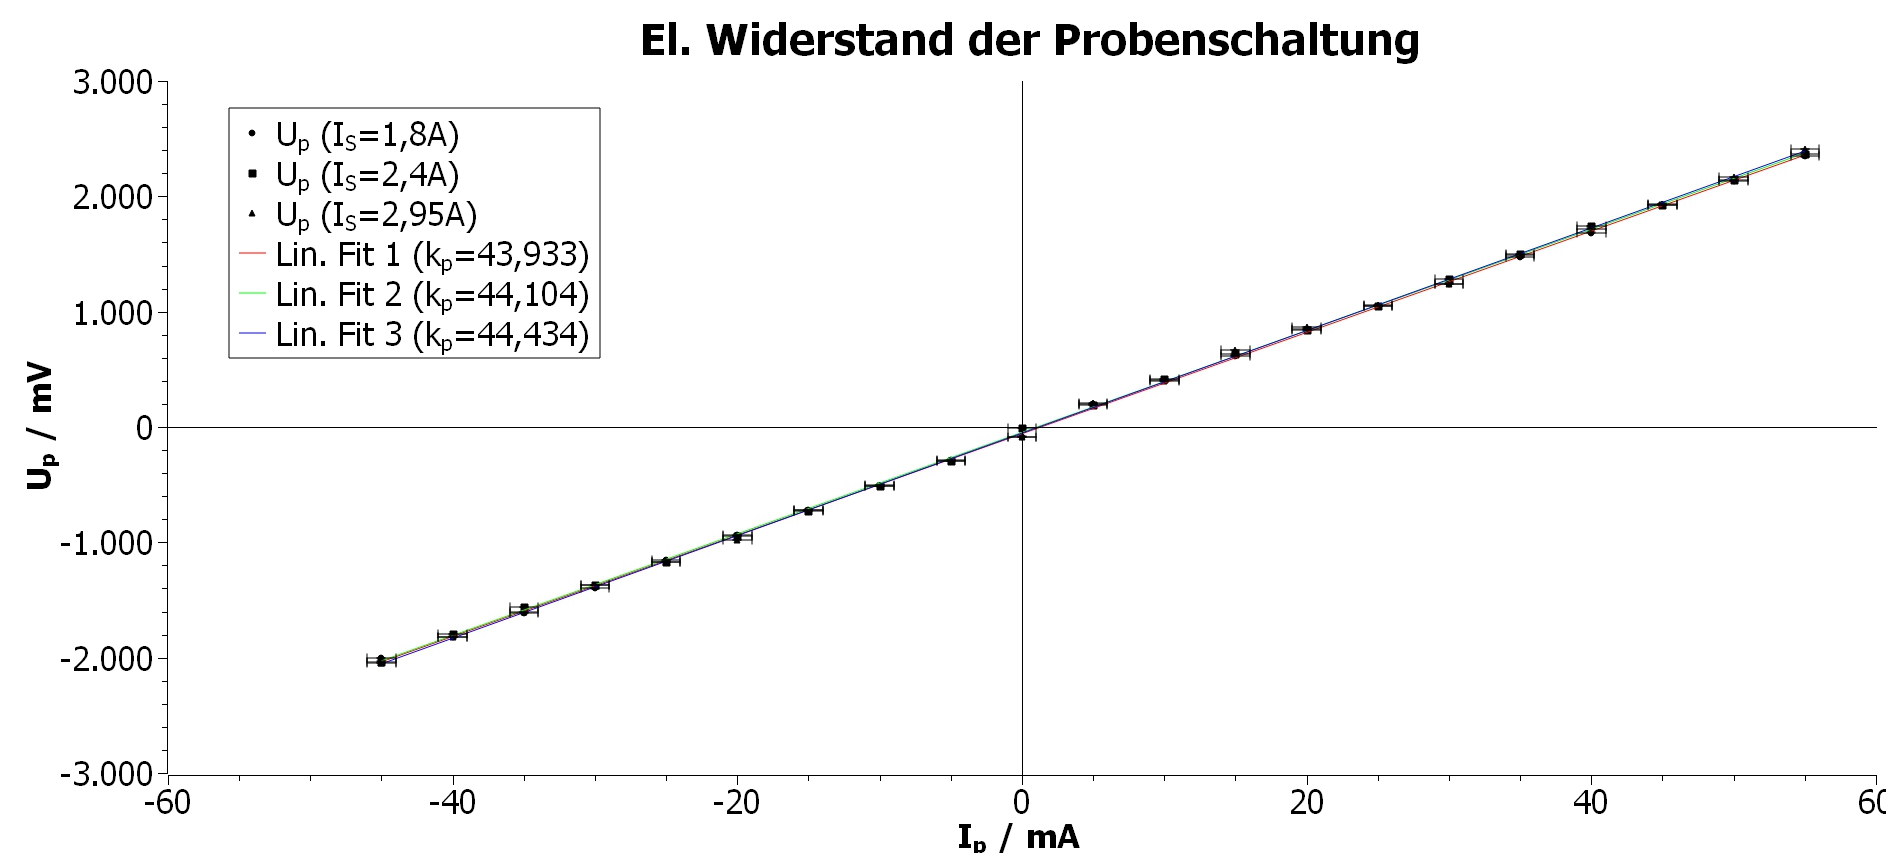
\includegraphics[width=\textwidth]{scidavis/abbildungen/R_probe.jpeg}
    \caption[Diagram der Messwerte \(U_p(I_p)\)]{Diagram der Messwerte \(U_p(I_p)\). Die Steigung des Linearen Fits \(k_p\) entspricht dem elektrischen Widerstand der Probenschaltung.}%
    \label{fig:Rprobe}
\end{figure}
Die Steigung des linearen Fits in \cref{fig:Rprobe} ist direkt als elektrischen Widerstand der Probe zu interpretieren.
Mit \cref{eq:spezR} lässt sich daraus der spezifische Widerstand \(\rho\)
\begin{equation}
    \rho = k_p \cdot \frac{b h}{l} = \SI{44,104}{\Omega} \cdot \frac{\SI{0,001}{m} \cdot \SI{0,01}{m}}{\SI{0,02}{m}} \approx \SI{0,022}{\Omega m}%
    \label{eq:spezRnum}
\end{equation}
und die Ladungsträgerbeweglichkeit \(\mu\) (nicht zu verwechseln mit der magnetischen Permeabilität) - ein Maß für
Driftgeschwindigkeit der Ladungsträger innerhalb eines elektrischen Feldes - innerhalb des Probenmaterials ermitteln.
\begin{equation}
    \mu = \frac{1}{\rho} \cdot A_H
    = \frac{1}{\SI{0,022}{\Omega m}}\cdot -\SI{5,54 \cdot 10^{-3}}{\metre\cubed\per\ampere\per\second}
    \approx -\SI{0,252}{\metre\squared\per\volt\second}
\end{equation}
%
\par
Die Fehler liegen hier bei
\begin{align}
    \Delta \rho &= \left| \frac{\partial \rho}{\partial k_p} \right| \cdot \Delta k_p +
    \left| \frac{\partial \rho}{\partial b} \right| \cdot \Delta b +
    \left| \frac{\partial \rho}{\partial h} \right| \cdot \Delta h +
    \left| \frac{\partial \rho}{\partial l} \right| \cdot \Delta l \nonumber \\
    &= \left| \frac{b \cdot h}{l} \right| \cdot \Delta k_p +
    \left| \frac{k_p \cdot h}{l} \right| \cdot \Delta b +
    \left| \frac{k_p \cdot b}{l} \right| \cdot \Delta h +
    \left| \frac{k_p \cdot b \cdot h}{l^2} \right| \cdot \Delta l \nonumber \\
    &= \left( \frac{\SI{10^{-3}}{m} \cdot \SI{10^{-2}}{m}}{2 \cdot \SI{10^{-2}}{m}} \right) \cdot \SI{0,136}{\volt\per\ampere} +
    \left( \frac{\SI{44,104}{\volt\per\ampere} \cdot \SI{10^{-2}}{m}}{2 \cdot \SI{10^{-2}}{m}} \right) \cdot \SI{10^{-4}}{m} \nonumber \\
    &\quad+ \left( \frac{\SI{44,104}{\volt\per\ampere} \cdot \SI{10^{-3}}{m}}{2 \cdot \SI{10^{-2}}{m}} \right) \cdot \SI{10^{-4}}{m} +
    \left( \frac{\SI{44,104}{\volt\per\ampere} \cdot \SI{10^{-3}}{m} \cdot \SI{10^{-2}}{m}}{4 \cdot \SI{10^{-4}}{m^2}} \right) \cdot \SI{10^{-4}}{m}\nonumber \\
    &= \pm 3 \cdot \SI{10^{-3}}{\Omega m}
\end{align}
und
\begin{align}
    \Delta \mu &=
    \left| \frac{\partial \mu}{\partial \rho} \right| \cdot \Delta \rho +
    \left| \frac{\partial \mu}{\partial A_H} \right| \cdot \Delta A_H \nonumber \\
    &=
    \left| \frac{A_H}{\rho^2} \right| \cdot \Delta \rho +
    \left| \rho^{-1} \right| \cdot \Delta A_H \nonumber \\
    &=
    \left( \frac{5,54 \cdot \SI{10^{-3}}{\metre\cubed\per\ampere\per\second}}{\left( \SI{0,022}{\Omega m} \right)^2} \right) \cdot 3 \cdot \SI{10^{-3}}{\Omega m} +
    \left( \SI{0,022}{\Omega m} \right)^{-1} \cdot 7,534 \cdot \SI{10^{-4}}{\Omega} \nonumber \\
    &= \pm \SI{0,069}{\metre\squared\per\volt\second}
\end{align}
\section{Messunsicherheiten}
\begin{table}[h]
    \centering
    \begin{tabular}{@{}ll@{}}
        \toprule
        Größe                                            & Wert                                                                    \\ \midrule
        \textsc{Hall}-Koeffizient $A_H$                  & \( (-5,54 \cdot 10^{-3} \pm 7,534 \cdot 10^{-4})\SI{}{\Omega}\)         \\
        Ladungsträgerdichte $n_q$                        & \( (1,128 \cdot 10^{21} \pm 1,173 \cdot 10^{20})\SI{}{m^{-3}}\)         \\
        Spezifischer Widerstand \(\rho\)                 & \( (0,022 \pm 3 \cdot 10^{-3})\SI{}{\Omega m} \)                        \\
        Ladungsträgerbeweglichkeit \(\mu\)               & \( (-0,252 \pm 0,069)\SI{}{\metre\squared\per\volt\second} \)                           \\ \bottomrule
    \end{tabular}
\end{table}